\documentclass{article}

\usepackage{arxiv}

\usepackage[utf8]{inputenc}   % entrada UTF-8 (acentos)
\usepackage[T1]{fontenc}      % fuentes de 8 bits
\usepackage[spanish,es-tabla,es-noshorthands,es-nodecimaldot]{babel}
\usepackage[table]{xcolor}    % colores (filas resaltadas en tablas)
\usepackage{hyperref}         % hipervínculos
\usepackage{url}              % URLs
\usepackage{booktabs}         % tablas profesionales
\usepackage{amsfonts}         % símbolos matemáticos
\usepackage{amsmath}          % ecuaciones
\usepackage{nicefrac}         % fracciones compactas
\usepackage{microtype}        % microtipografía
\usepackage{graphicx}         % figuras
\usepackage{array}            % columnas con formato
\usepackage{placeins}         % \FloatBarrier
\usepackage[numbers,sort&compress]{natbib} % citas numéricas (\cite, \citet)
\usepackage{caption}          % leyendas
\captionsetup{font=small, labelfont=bf}
\hypersetup{colorlinks=true, linkcolor=blue!50!black, citecolor=blue!50!black,
            urlcolor=blue!50!black}
\graphicspath{{../figures/}}

% Etiquetas del template arxiv.sty traducidas al español (el estilo no se modifica)
\def\keywordname{{\bfseries \emph{Palabras clave}}}
\renewenvironment{abstract}
  {\centerline{\large \bfseries \scshape Resumen}\begin{quote}}
  {\end{quote}}
\rhead{\scshape Trabajo práctico - UCA - \today}

% Cifras generadas automáticamente por el código R (results/numeros.tex).
% Así cada número del informe coincide exactamente con lo que produce el código.
\newcommand{\nTotal}{215.845}
\newcommand{\nTrain}{143.892}
\newcommand{\nTest}{71.953}
\newcommand{\nDefault}{27.796}
\newcommand{\tasaTotal}{12,9\%}
\newcommand{\tasaTrain}{12,7\%}
\newcommand{\tasaTest}{13,2\%}
\newcommand{\montoTotal}{2,69~mil millones}
\newcommand{\tasaGradoA}{5,6\%}
\newcommand{\tasaGradoG}{20,5\%}
\newcommand{\corrCuotaMonto}{0,99}
\newcommand{\nCandidatas}{33}
\newcommand{\nDescIV}{17}
\newcommand{\nDescCor}{3}
\newcommand{\nFinales}{17}
\newcommand{\nColumnasX}{27}
\newcommand{\nAjuste}{84.594}
\newcommand{\nValid}{59.298}
\newcommand{\ivSubgrado}{0,228}
\newcommand{\ivTasa}{0,227}
\newcommand{\rfMtry}{3}
\newcommand{\rfNodo}{200}
\newcommand{\gbmProf}{5}
\newcommand{\gbmArboles}{200}
\newcommand{\lassoCeros}{15}
\newcommand{\lassoTotal}{27}
\newcommand{\aucFuga}{0,9998}
\newcommand{\mejorModelo}{Gradient Boosting}
\newcommand{\aucBench}{0,649}
\newcommand{\aucValidBench}{0,647}
\newcommand{\giniBench}{0,298}
\newcommand{\ksBench}{0,220}
\newcommand{\sensBench}{0,633}
\newcommand{\especBench}{0,586}
\newcommand{\accBench}{0,592}
\newcommand{\precBench}{0,189}
\newcommand{\fUnoBench}{0,291}
\newcommand{\umbralBench}{0,121}
\newcommand{\brierBench}{0,1114}
\newcommand{\aucLogit}{0,668}
\newcommand{\aucValidLogit}{0,666}
\newcommand{\giniLogit}{0,335}
\newcommand{\ksLogit}{0,249}
\newcommand{\sensLogit}{0,657}
\newcommand{\especLogit}{0,590}
\newcommand{\accLogit}{0,599}
\newcommand{\precLogit}{0,196}
\newcommand{\fUnoLogit}{0,302}
\newcommand{\umbralLogit}{0,117}
\newcommand{\brierLogit}{0,1102}
\newcommand{\aucLasso}{0,667}
\newcommand{\aucValidLasso}{0,668}
\newcommand{\giniLasso}{0,335}
\newcommand{\ksLasso}{0,249}
\newcommand{\sensLasso}{0,619}
\newcommand{\especLasso}{0,629}
\newcommand{\accLasso}{0,627}
\newcommand{\precLasso}{0,203}
\newcommand{\fUnoLasso}{0,305}
\newcommand{\umbralLasso}{0,127}
\newcommand{\brierLasso}{0,1102}
\newcommand{\aucRF}{0,666}
\newcommand{\aucValidRF}{0,666}
\newcommand{\giniRF}{0,333}
\newcommand{\ksRF}{0,248}
\newcommand{\sensRF}{0,696}
\newcommand{\especRF}{0,548}
\newcommand{\accRF}{0,568}
\newcommand{\precRF}{0,190}
\newcommand{\fUnoRF}{0,299}
\newcommand{\umbralRF}{0,121}
\newcommand{\brierRF}{0,1101}
\newcommand{\aucGBM}{0,670}
\newcommand{\aucValidGBM}{0,669}
\newcommand{\giniGBM}{0,339}
\newcommand{\ksGBM}{0,251}
\newcommand{\sensGBM}{0,684}
\newcommand{\especGBM}{0,565}
\newcommand{\accGBM}{0,581}
\newcommand{\precGBM}{0,193}
\newcommand{\fUnoGBM}{0,302}
\newcommand{\umbralGBM}{0,119}
\newcommand{\brierGBM}{0,1100}
\newcommand{\aucMejor}{0,670}
\newcommand{\aucValidMejor}{0,669}
\newcommand{\giniMejor}{0,339}
\newcommand{\ksMejor}{0,251}
\newcommand{\sensMejor}{0,684}
\newcommand{\especMejor}{0,565}
\newcommand{\accMejor}{0,581}
\newcommand{\precMejor}{0,193}
\newcommand{\fUnoMejor}{0,302}
\newcommand{\umbralMejor}{0,119}
\newcommand{\brierMejor}{0,1100}
\newcommand{\pDelongBench}{$1{,}6 \times 10^{-35}$}
\newcommand{\pDelongLogit}{0,005}
\newcommand{\corrTasaPD}{0,86}
\newcommand{\retTodos}{9,83\%}
\newcommand{\retMejorSetenta}{10,00\%}
\newcommand{\retBenchSetenta}{9,49\%}
\newcommand{\defMejorSetenta}{9,4\%}
\newcommand{\defBenchSetenta}{10,1\%}
\newcommand{\ganMejorSetenta}{67,5~millones}
\newcommand{\ganBenchSetenta}{63,3~millones}
\newcommand{\ganTodos}{89,9~millones}
\newcommand{\difGanSetenta}{4,3~millones}

% Las tablas se insertan con el \input primitivo de TeX: el \input de LaTeX
% rompe las reglas de booktabs (\bottomrule) dentro de un tabular.
\makeatletter
\newcommand{\tablainput}[1]{\@@input #1 }
\makeatother

\title{¿Quién no va a devolver el préstamo?\\[0.3em]
\large Predicción de incumplimiento crediticio con datos reales de LendingClub,
validación fuera de tiempo y análisis económico}

\author{
  Matías Costabile \\
  Licenciatura en Ciencia de Datos\\
  Pontificia Universidad Católica Argentina (UCA)\\
  Buenos Aires, Argentina \\
  \texttt{matycostabile2008@gmail.com} \\
}

\begin{document}
\maketitle

\begin{abstract}
Un préstamo que no se devuelve es plata que se pierde. Este trabajo construye y
evalúa modelos que estiman, \emph{en el momento de la solicitud}, la probabilidad
de que un préstamo personal termine en incumplimiento (\emph{default}). Se usan
\nTotal{} préstamos reales a 36 meses de la plataforma estadounidense LendingClub
emitidos entre 2012 y mediados de 2014, todos con resultado final conocido
(tasa de default: \tasaTotal). Se aplica un proceso completo de extracción,
transformación, imputación e ingeniería de características, y una selección
basada en \emph{Information Value} y correlación. Se comparan cinco modelos
---un \emph{benchmark} que usa sólo la calificación de la propia plataforma,
regresión logística, LASSO, Random Forest y Gradient Boosting--- con una
partición \emph{fuera de tiempo}: se entrena con 2012--2013 y se evalúa con
2014. El mejor modelo (\mejorModelo) alcanza un AUC de \aucMejor{} en prueba,
frente a \aucBench{} de la calificación de LendingClub (test de DeLong,
$p = $ \pDelongBench). Aprobando el 70\% de las solicitudes, el modelo baja la
tasa de default de la cartera de \defBenchSetenta{} a \defMejorSetenta{} y sube
su retorno real de \retBenchSetenta{} a \retMejorSetenta{}. Además, se muestra
empíricamente que incluir variables posteriores al otorgamiento produce un AUC
engañoso de \aucFuga, lo que obliga a leer con cautela resultados casi
perfectos reportados en la literatura.
\end{abstract}

\keywords{Riesgo de crédito \and Credit scoring \and LendingClub \and
Préstamos P2P \and Gradient Boosting \and Regresión logística \and
Fuga de información}

% =====================================================================
\section{Objetivo}
\label{sec:objetivo}

\paragraph{Objetivo general.} Desarrollar un modelo de clasificación que estime,
con la información disponible el día en que se pide un préstamo, la probabilidad
de que el solicitante no lo devuelva, y medir si ese modelo mejora las decisiones
de crédito respecto de la calificación que ya asigna la plataforma.

\paragraph{Objetivos específicos.}
\begin{enumerate}
  \item Construir un conjunto de datos libre de \emph{fuga de información}
        (\emph{data leakage}): sólo variables conocidas al originar el préstamo.
  \item Diseñar las características óptimas mediante extracción, transformación,
        imputación, ingeniería y selección de variables.
  \item Entrenar y comparar cinco modelos de clasificación con métricas
        estadísticas (AUC, Gini, KS, Brier, sensibilidad, especificidad,
        precisión, F1, \emph{accuracy}) bajo una validación fuera de tiempo.
  \item Traducir el desempeño estadístico a dinero: retorno real de la cartera
        aprobada según cada criterio.
  \item Comparar los resultados con al menos cinco trabajos del estado del arte
        que usaron la misma fuente de datos.
\end{enumerate}

% =====================================================================
\section{Introducción}
\label{sec:intro}

\subsection{Contexto}
Los préstamos \emph{peer-to-peer} (P2P) conectan a personas que necesitan dinero
con inversores que lo prestan, a través de una plataforma en línea y sin un banco
de por medio. LendingClub fue durante años la plataforma P2P más grande de Estados
Unidos y publicó el historial completo de sus préstamos, lo que la convirtió en
una de las fuentes más usadas para investigar riesgo de crédito. En este esquema
el riesgo lo asume el inversor, que dispone de mucha menos información que el
solicitante (\emph{asimetría de información}). Por eso la plataforma asigna a
cada préstamo un \emph{grado} (A a G, con sub-grados A1 a G5) que determina la
tasa de interés.

La pregunta central de este trabajo es concreta: \emph{¿se puede predecir mejor
que la propia plataforma quién no va a devolver el préstamo, y cuánto vale esa
mejora en dinero?}

\subsection{Resumen del trabajo}
Se partió de los datos públicos de LendingClub y se seleccionaron los
\nTotal{} préstamos a 36 meses emitidos entre enero de 2012 y junio de 2014 cuyo
estado final es conocido (\emph{Fully Paid} o \emph{Charged Off}), por un total
de US\$\montoTotal. Se definió como variable objetivo el incumplimiento y se
separaron estrictamente las variables conocidas al originar el préstamo de las
que describen cómo se pagó. Luego se aplicó un proceso de ingeniería de
características cuyos parámetros se aprenden sólo del entrenamiento, se entrenaron
cinco modelos y se los evaluó una única vez sobre préstamos de 2014, que el
modelo nunca vio y que corresponden a un período posterior. Finalmente se
cuantificó el impacto económico y se ilustró el efecto de la fuga de información.

\subsection{Estado del arte}
\label{sec:estado-arte}

La literatura sobre LendingClub coincide en tres hallazgos: el grado asignado por
la plataforma es la variable individual más predictiva, el endeudamiento y el
ingreso del solicitante aportan información adicional, y la capacidad
discriminante alcanzable con datos de originación es moderada (AUC cercano a
0,70). La Tabla~\ref{tab:estado-arte} resume ocho trabajos.

\citet{emekter2015} analizaron préstamos de LendingClub con
regresión logística y modelos de supervivencia de Cox. Encontraron que el grado,
la relación deuda/ingreso, el puntaje FICO y el uso del crédito rotativo explican
el incumplimiento, y que las tasas más altas cobradas a los solicitantes riesgosos
no alcanzan a compensar su mayor probabilidad de default.

\citet{serrano2015} estudiaron 24.449 préstamos (2008--2014) y desarrollaron una
regresión logística. El grado resultó el factor más predictivo, y agregar
información del solicitante (sobre todo su nivel de deuda) mejoró el modelo. En
su muestra de prueba (3.788 préstamos de 2011) reportan una tasa de acierto de
75,2\% con sólo el sub-grado y de 65,1\% con el modelo completo. Esta inversión
aparente ilustra que el \emph{accuracy} depende del umbral y del balance de
clases, y por eso no sirve para comparar modelos en este problema.

\citet{malekipirbazari2015} compararon Random Forest, regresión logística, $k$
vecinos más cercanos y máquinas de soporte vectorial. Random Forest fue el mejor
clasificador y superó tanto al puntaje FICO como al grado de LendingClub para
identificar buenos pagadores.

\citet{xia2017} propusieron un XGBoost sensible al costo, que penaliza más
aprobar a un mal pagador que rechazar a uno bueno, y mostraron que los modelos
que ignoran los costos pueden llevar incluso a retornos negativos. Señalaron que
las variables que predicen el default no son las mismas que predicen la
rentabilidad, una idea que este trabajo confirma en la Sección~\ref{sec:res-eco}.

\citet{ma2018} aplicaron LightGBM y XGBoost a datos de LendingClub con distintas
estrategias de limpieza. LightGBM fue el mejor y, según sus cálculos, mejorar 1,28
puntos porcentuales la tasa de acierto habría evitado unos US\$117 millones en
préstamos incumplidos.

\citet{namvar2018} usaron 66.376 préstamos de 2016--2017 (18,3\% de default),
eliminaron explícitamente el grado y la tasa de interés, e introdujeron un
``DTI nuevo'' que incluye la cuota del préstamo solicitado (idea que se adopta en
este trabajo). Combinando clasificadores con técnicas de remuestreo obtuvieron
AUC entre 0,69 y 0,71. La regresión logística sin remuestreo logró AUC = 0,703,
pero con una especificidad de sólo 4,8\%, porque casi todo lo predecía como
``pagó''.

\citet{turiel2020} entrenaron regresión logística, máquinas de soporte vectorial y
redes neuronales profundas sobre unos 800.000 préstamos (2007--2017) con una
partición temporal. Para predecir el default obtuvieron AUC = 0,69 con regresión
logística y con la mejor red neuronal, y 0,643 con máquinas de soporte vectorial.

Por último, \citet{gupta2022} reportan AUC de 0,910 (regresión logística) y
0,928 (Random Forest), con \emph{accuracy} de 97,1\% en prueba y de 100\% en
entrenamiento. Esos valores están muy por encima del resto de la literatura y el
trabajo no documenta explícitamente la exclusión de las variables posteriores al
otorgamiento. La Sección~\ref{sec:res-fuga} muestra que, con datos de LendingClub,
incluir ese tipo de variables produce justamente métricas casi perfectas.

\begin{table}[htbp]
\caption{Trabajos del estado del arte con datos de LendingClub. N/R: no reportado
en una métrica comparable. Los valores corresponden al conjunto de prueba
informado por cada trabajo.}
\label{tab:estado-arte}
\centering
\small
\begin{tabular}{>{\raggedright\arraybackslash}p{2.7cm}>{\raggedright\arraybackslash}p{2.3cm}>{\raggedright\arraybackslash}p{4.0cm}>{\raggedright\arraybackslash}p{4.6cm}}
\toprule
Trabajo & Datos & Métodos & Resultado principal \\
\midrule
\citet{emekter2015} & LendingClub & Logit, Cox & Grado, DTI, FICO y uso del rotativo explican el default \\
\citet{serrano2015} & 2008--2014; 24.449 & Logit & Accuracy 75,2\% (sub-grado) y 65,1\% (completo) \\
\citet{malekipirbazari2015} & LendingClub & RF, Logit, $k$-NN, SVM & RF supera a FICO y al grado de LC \\
\citet{xia2017} & 49.795 & XGBoost sensible al costo & Mejor rentabilidad que modelos sin costos \\
\citet{ma2018} & 480.018 & LightGBM, XGBoost & LightGBM mejor (+1,28 p.p. de acierto) \\
\citet{namvar2018} & 2016--2017; 66.376 & Logit, LDA, RF + remuestreo & AUC 0,69--0,71 \\
\citet{turiel2020} & 2007--2017; $\sim$800.000 & Logit, SVM, redes neuronales & AUC 0,69 (Logit y red) \\
\citet{gupta2022} & Kaggle, todos los años & Logit, RF & AUC 0,91--0,93 (posible fuga) \\
\midrule
\textbf{Este trabajo} & 2012--2014; \nTotal & Logit, LASSO, RF, GBM & \textbf{AUC \aucMejor{} fuera de tiempo} \\
\bottomrule
\end{tabular}
\end{table}

\subsection{Aportes de este trabajo}
Respecto de los trabajos anteriores, este trabajo combina cuatro elementos que
rara vez aparecen juntos: (i) una validación estrictamente fuera de tiempo, con
selección de hiperparámetros y umbral también fuera de tiempo; (ii) un
\emph{benchmark} explícito contra la calificación de la plataforma, con test
estadístico de la diferencia; (iii) una evaluación económica con el dinero
efectivamente cobrado, y (iv) una demostración cuantitativa del efecto de la fuga
de información. Todo el código es reproducible y cada cifra del informe se genera
automáticamente desde él.

% =====================================================================
\section{Datos}
\label{sec:datos}

\paragraph{Fuente.} Datos públicos de préstamos emitidos por LendingClub, en la
versión empaquetada por \citet{kuhn2017data} (foto de la cartera de fines de
2017). Se usó R \cite{rcore2023}.

\paragraph{Población.} Préstamos a 36 meses emitidos entre 2012-01 y 2014-06. Se
eligió ese recorte por dos motivos. Primero, a fines de 2017 todos esos préstamos
ya vencieron, así que su resultado es definitivo (se descartaron sólo 2 préstamos
todavía en mora). Incluir préstamos más nuevos obligaría a excluir los que siguen
vigentes, y eso sesgaría la muestra hacia los que fallaron rápido. Segundo, mezclar
plazos de 36 y 60 meses junta dos productos con riesgos muy distintos.

\paragraph{Variable objetivo.}
\begin{equation}
y_i = \begin{cases} 1 & \text{si el préstamo } i \text{ terminó en \emph{Charged Off} (default)} \\
0 & \text{si fue \emph{Fully Paid}} \end{cases}
\end{equation}

\paragraph{Variables.} El archivo tiene 36 columnas: 30 conocidas al originar el
préstamo (monto, tasa, cuota, grado y sub-grado, antigüedad laboral, vivienda,
ingreso, verificación del ingreso, propósito, estado, DTI, historial de atrasos,
consultas recientes, cuentas abiertas y totales, saldo y uso del crédito
rotativo, quiebras, hipotecas, saldos totales, etc.), la variable de estado y 5
variables \emph{posteriores} (monto financiado, total pagado, capital devuelto,
recuperos y último pago). Estas últimas \textbf{nunca} se usan como predictoras:
sólo sirven para el análisis económico y el experimento de fuga.

\paragraph{Partición fuera de tiempo.} La Tabla~\ref{tab:particion} muestra los
tres conjuntos. Las decisiones de modelado (hiperparámetros, umbral) se toman con
\emph{ajuste} y \emph{validación}. Con lo elegido se re-entrena sobre todo 2012--2013
y se evalúa \emph{una única vez} sobre 2014. Una partición aleatoria mezclaría
préstamos de distintos momentos del ciclo económico y daría una estimación
optimista: en la práctica, un modelo siempre se usa sobre clientes futuros.

\begin{table}[htbp]
\caption{Partición temporal de los datos.}
\label{tab:particion}
\centering
\begin{tabular}{llrr}
\toprule
Conjunto & Período de emisión & Préstamos & Uso \\
\midrule
Ajuste      & 2012-01 a 2013-06 & \nAjuste & Aprender transformaciones y modelos \\
Validación  & 2013-07 a 2013-12 & \nValid  & Elegir hiperparámetros y umbral \\
\midrule
Entrenamiento (ajuste + validación) & 2012-01 a 2013-12 & \nTrain & Modelo final (tasa default \tasaTrain) \\
Prueba      & 2014-01 a 2014-06 & \nTest   & Evaluación final (tasa default \tasaTest) \\
\bottomrule
\end{tabular}
\end{table}

% =====================================================================
\section{Metodología}
\label{sec:metodologia}

\subsection{Prevención de la fuga de información}
Hay fuga de información cuando un modelo usa, al entrenarse, datos que no estarán
disponibles al momento de predecir \cite{kaufman2012}. En crédito, el caso típico
es usar variables de pago (cuánto se devolvió, si hubo recuperos): contienen la
respuesta. La regla aplicada en todo el trabajo es doble. Primero, sólo entran
variables conocidas al originar el préstamo. Segundo, todo parámetro que se
aprende de los datos (percentiles, medianas, medias, desvíos, WoE) se estima
\emph{sólo} con el conjunto de ajuste y luego se aplica, sin recalcular, a
validación y prueba.

\subsection{Extracción de características}
A partir de las columnas originales se crearon variables nuevas con sentido
financiero:
\begin{align}
\text{antigüedad\_crédito}_i &= \text{meses entre la primera línea de crédito y la emisión} \\
\text{subgrado\_num}_i &= 5\,(\text{letra}_i - 1) + \text{número}_i \in \{1,\dots,35\} \quad (\text{A1}=1,\ \text{G5}=35)\\
\text{cuota\_ingreso}_i &= \frac{12 \cdot \text{cuota}_i}{\text{ingreso anual}_i} \\
\text{dti\_con\_préstamo}_i &= \text{DTI}_i + 100 \cdot \text{cuota\_ingreso}_i \label{eq:dti}\\
\text{préstamo\_ingreso}_i &= \frac{\text{monto}_i}{\text{ingreso anual}_i}, \qquad
\text{ratio\_cuentas\_abiertas}_i = \frac{\text{cuentas abiertas}_i}{\text{cuentas totales}_i}
\end{align}
La ecuación~\eqref{eq:dti} corrige una limitación del DTI que publica LendingClub,
que no incluye la cuota del préstamo que se está pidiendo \cite{namvar2018}. La
antigüedad laboral, que viene como texto (``10+ years''), se convirtió a número
de años.

\subsection{Transformación}
\begin{itemize}
  \item \textbf{Recorte de extremos (winsorización).} Hay ingresos declarados de
        hasta US\$7,4 millones. Cada variable numérica se recorta a los
        percentiles 1 y 99 del ajuste: $\tilde{x} = \min(\max(x, q_{0,01}), q_{0,99})$.
  \item \textbf{Logaritmo.} A las variables muy asimétricas (ingreso, saldos) se
        les aplica $\log(1+x)$.
  \item \textbf{Categorías raras.} En las variables categóricas, los niveles con
        menos de 1\% de frecuencia se agrupan en ``OTRA''.
  \item \textbf{Codificación WoE.} El estado de residencia (50 categorías) se
        reemplaza por su \emph{Weight of Evidence}, ecuación~\eqref{eq:woe}, en
        lugar de crear 50 variables binarias.
  \item \textbf{Estandarización} (para los modelos lineales):
        $z = (x - \bar{x}_{\text{ajuste}}) / s_{\text{ajuste}}$. Las
        categóricas se convierten en variables indicadoras.
\end{itemize}

\subsection{Imputación}
Se distinguieron dos mecanismos de dato faltante, y en ambos casos se agregó una
variable indicadora $\mathbb{1}[x_i \text{ faltante}]$ para no perder la
información que aporta la ausencia misma:
\begin{itemize}
  \item \textbf{Imputación estructural.} En ``meses desde el último atraso''
        (57\% faltante en entrenamiento), el dato falta porque el cliente \emph{nunca} se
        atrasó. Rellenar con la mediana sería un error conceptual, así que se
        imputa el máximo observado (``hace muchísimo tiempo'').
  \item \textbf{Imputación estadística por mediana.} En saldos totales, límite
        de crédito rotativo, cantidad de hipotecas, uso del rotativo y
        antigüedad laboral, el dato falta porque no se registró (por ejemplo,
        durante buena parte de 2012 LendingClub no informaba los saldos totales).
        Se imputa la mediana del ajuste.
\end{itemize}

\subsection{Selección de características}
\paragraph{Paso 1: Information Value.} Para cada variable se forman grupos (deciles
si es numérica, categorías si es categórica, y un grupo propio para los faltantes)
y se calcula
\begin{equation}
\text{WoE}_g = \ln\!\left(\frac{\%\,\text{buenos}_g}{\%\,\text{malos}_g}\right),
\qquad
\text{IV} = \sum_{g} \left(\%\,\text{buenos}_g - \%\,\text{malos}_g\right)\,\text{WoE}_g ,
\label{eq:woe}
\end{equation}
donde $\%\,\text{buenos}_g$ es la fracción de todos los préstamos pagados que cae en
el grupo $g$. Siguiendo la escala usual en \emph{scoring} crediticio
\cite{siddiqi2006}, se descartan las variables con IV $< 0{,}02$.

\paragraph{Paso 2: filtro de correlación.} Si dos variables numéricas tienen
$|r| > 0{,}85$, aportan casi la misma información y generan multicolinealidad. Se
conserva la de mayor IV.

\paragraph{Paso 3: selección embebida (LASSO).} La penalización $L_1$ del modelo
LASSO (ecuación~\ref{eq:lasso}) lleva a cero los coeficientes de las variables
que no aportan.

\subsection{Modelos}

\paragraph{M0: Benchmark.} Regresión logística con una sola variable, el sub-grado
de LendingClub. Representa lo que ya sabe la plataforma: cualquier modelo útil
debe superarlo.

\paragraph{M1: Regresión logística} \cite{hosmer2013}. Modela la probabilidad de
default como
\begin{equation}
p_i = P(y_i = 1 \mid \mathbf{x}_i) = \frac{1}{1 + e^{-(\beta_0 + \boldsymbol{\beta}^\top \mathbf{x}_i)}}
\end{equation}
y estima $\boldsymbol\beta$ maximizando la log-verosimilitud
\begin{equation}
\ell(\boldsymbol\beta) = \sum_{i=1}^{n} \left[ y_i \ln p_i + (1-y_i)\ln(1-p_i) \right].
\end{equation}
Con variables estandarizadas, $e^{\beta_j}$ es el \emph{odds ratio} asociado a un
aumento de un desvío estándar en $x_j$.

\paragraph{M2: LASSO logístico} \cite{tibshirani1996,friedman2010}.
\begin{equation}
\hat{\boldsymbol\beta} = \arg\min_{\boldsymbol\beta} \; -\frac{1}{n}\,\ell(\boldsymbol\beta)
+ \lambda \sum_{j=1}^{p} |\beta_j| .
\label{eq:lasso}
\end{equation}
$\lambda$ se elige por validación cruzada de 5 particiones maximizando el AUC, y
se toma el $\lambda$ más grande a un error estándar del óptimo (regla
\emph{1-SE}) para favorecer un modelo más simple.

\paragraph{M3: Random Forest} \cite{breiman2001,wright2017}. Promedia $B$ árboles
de clasificación, cada uno entrenado sobre una muestra \emph{bootstrap} y
eligiendo en cada división entre $m$ variables al azar:
$\hat{p}(\mathbf{x}) = \frac{1}{B}\sum_{b=1}^{B} \hat{p}_b(\mathbf{x})$. Se buscó
$m \in \{3,5\}$ y tamaño mínimo de nodo $\in \{50, 200\}$. Se eligieron $m=\rfMtry$
y nodo mínimo $=\rfNodo$, y el modelo final usa $B=500$.

\paragraph{M4: Gradient Boosting} \cite{friedman2001}. Construye el modelo de forma
aditiva. Cada árbol nuevo $h_m$ se ajusta a los pseudo-residuos del modelo
anterior, que para la pérdida logística son $r_i = y_i - \hat p_i$:
\begin{equation}
F_m(\mathbf{x}) = F_{m-1}(\mathbf{x}) + \nu \, h_m(\mathbf{x}), \qquad
\hat{p}(\mathbf{x}) = \frac{1}{1+e^{-F_M(\mathbf{x})}} ,
\end{equation}
con tasa de aprendizaje $\nu = 0{,}03$ y submuestreo de 80\%. La profundidad
($\{3,5\}$) y la cantidad de árboles ($100$ a $1000$) se eligieron por AUC en
validación: profundidad \gbmProf{} y \gbmArboles{} árboles
(Figura~\ref{fig:tuning}).

\subsection{Desbalance de clases y umbral de decisión}
Sólo el \tasaTotal{} de los préstamos son default. En lugar de remuestrear los
datos, lo que distorsiona las probabilidades, se entrenó con la distribución real
y se ajustó el \emph{umbral} de decisión. Se clasifica como default si
$\hat p_i \geq c$, donde $c$ maximiza en \emph{validación} el índice de Youden
\cite{youden1950}:
\begin{equation}
J(c) = \text{Sensibilidad}(c) + \text{Especificidad}(c) - 1 .
\end{equation}

\subsection{Métricas de evaluación}
Con la clase positiva ``default'' y la matriz de confusión ($TP$, $FP$, $TN$,
$FN$):
\begin{align}
\text{Accuracy} &= \frac{TP+TN}{TP+FP+TN+FN}, &
\text{Sensibilidad} &= \frac{TP}{TP+FN}, &
\text{Especificidad} &= \frac{TN}{TN+FP}, \\
\text{Precisión} &= \frac{TP}{TP+FP}, &
F_1 &= \frac{2 \cdot \text{Precisión}\cdot\text{Sensibilidad}}{\text{Precisión}+\text{Sensibilidad}} .
\end{align}
Las métricas que no dependen del umbral son las principales:
\begin{itemize}
  \item \textbf{AUC} \cite{fawcett2006}: área bajo la curva ROC. Equivale a la
        probabilidad de que un default elegido al azar reciba un score mayor que
        un buen pagador elegido al azar, $\text{AUC}=P(\hat p_{\text{default}} > \hat p_{\text{pagó}})$.
        Su intervalo de confianza y la comparación entre modelos se hacen con el
        método de DeLong \cite{delong1988,robin2011}.
  \item \textbf{Gini} $= 2\,\text{AUC} - 1$, la forma en que la banca suele
        reportar el AUC.
  \item \textbf{KS} $= \max_s |F_{\text{pagó}}(s) - F_{\text{default}}(s)|$: máxima
        separación entre las distribuciones acumuladas de scores de ambas clases.
  \item \textbf{Brier} \cite{brier1950} $= \frac{1}{n}\sum_i (\hat p_i - y_i)^2$:
        error cuadrático de las probabilidades (mide calibración y discriminación).
\end{itemize}

\subsection{Evaluación económica}
\label{sec:met-eco}
Para cada tasa de aprobación $a \in \{10\%, 20\%, \dots, 100\%\}$ se aprueban los
préstamos con menor riesgo estimado y se calcula el retorno real a tres años de
esa cartera $\mathcal{A}_a$ con lo que efectivamente se cobró:
\begin{equation}
R(a) = \frac{\sum_{i \in \mathcal{A}_a} \text{total pagado}_i}{\sum_{i \in \mathcal{A}_a} \text{monto financiado}_i} - 1 .
\end{equation}
Se compara contra aprobar por sub-grado de LendingClub y contra aprobar al azar.
El retorno es bruto: no descuenta la comisión de la plataforma ni el costo de
fondeo.

% =====================================================================
\section{Resultados}
\label{sec:resultados}

\subsection{Análisis exploratorio}

La Figura~\ref{fig:temporal} muestra la tasa de default por mes de emisión y la
partición. La tasa se mantiene estable en el período (entre 12\% y 16\%), lo que
indica que no hay un cambio drástico de población entre entrenamiento y prueba.

\begin{figure}[htbp]
  \centering
  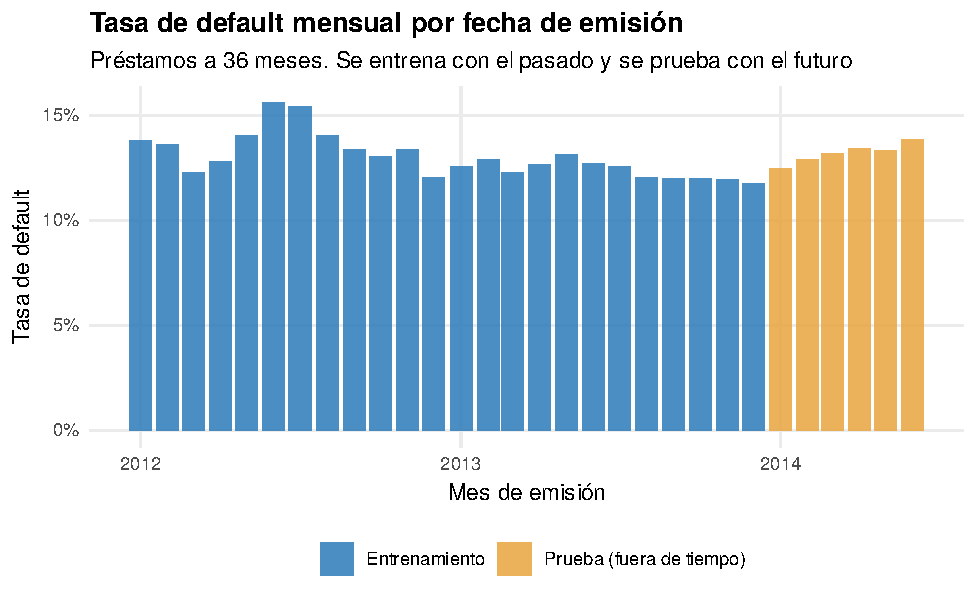
\includegraphics[width=0.85\textwidth]{eda_default_temporal.pdf}
  \caption{Tasa de default mensual por fecha de emisión y partición temporal.}
  \label{fig:temporal}
\end{figure}

La Figura~\ref{fig:grado} confirma que el grado de LendingClub ordena muy bien el
riesgo. La tasa de default sube de \tasaGradoA{} en el grado A a más de 25\% en
el F. El grado G casi no tiene préstamos a 36 meses en este período, por eso su
tasa es poco confiable. Este ordenamiento es el \emph{benchmark} a superar.

\begin{figure}[htbp]
  \centering
  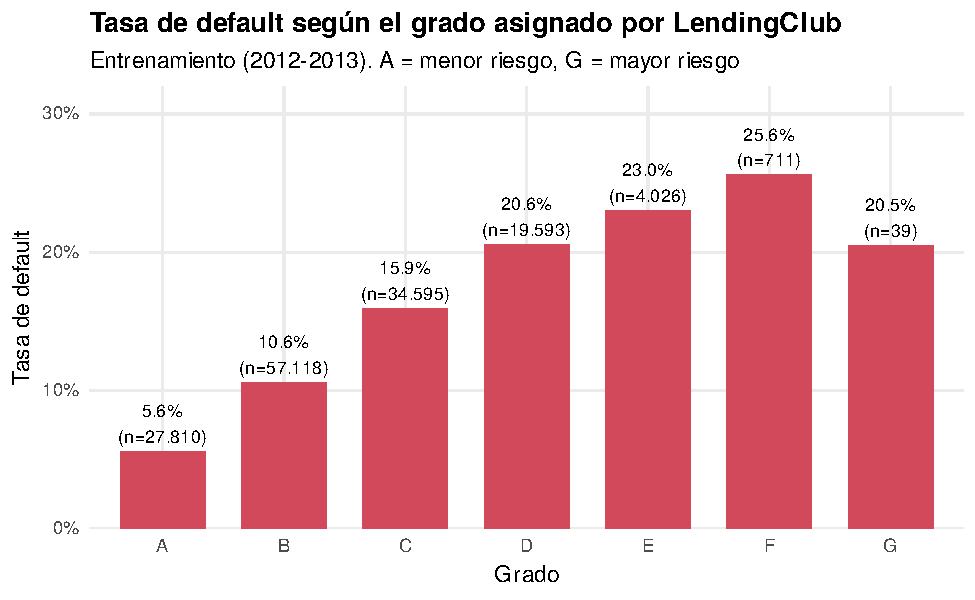
\includegraphics[width=0.8\textwidth]{eda_default_por_grado.pdf}
  \caption{Tasa de default según el grado asignado por LendingClub (entrenamiento).}
  \label{fig:grado}
\end{figure}

Los diagramas de dispersión de la Figura~\ref{fig:scatter-eda} muestran el
problema central: los defaults (rojo) no forman un grupo separado, sino que están
mezclados con los buenos pagadores. Se concentran algo más en tasas de interés
altas, ingresos bajos y DTI alto, pero con mucha superposición. Esto anticipa que
ningún modelo podrá separar perfectamente las clases con datos de originación.

\begin{figure}[htbp]
  \centering
  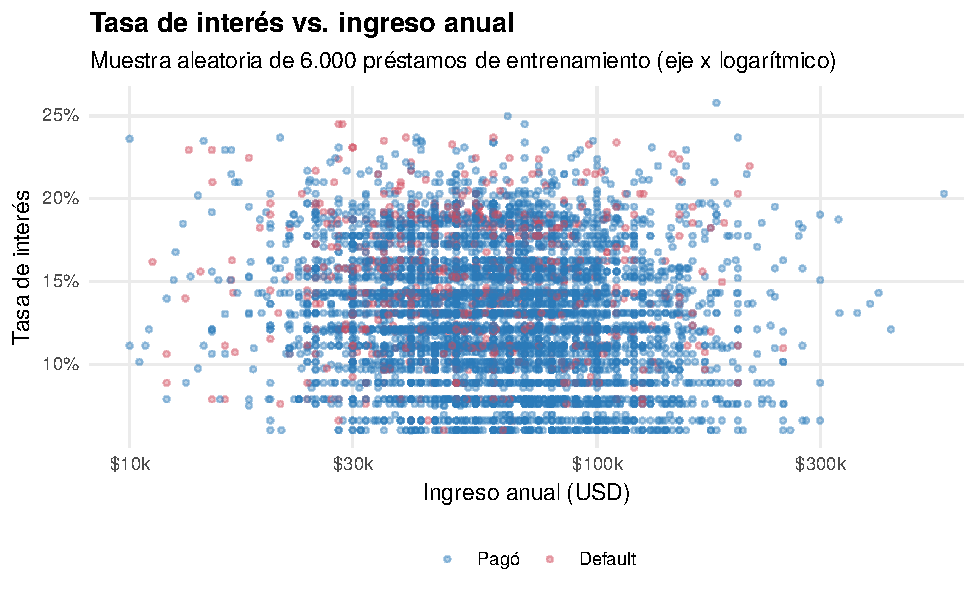
\includegraphics[width=0.49\textwidth]{eda_scatter_tasa_ingreso.pdf}
  \hfill
  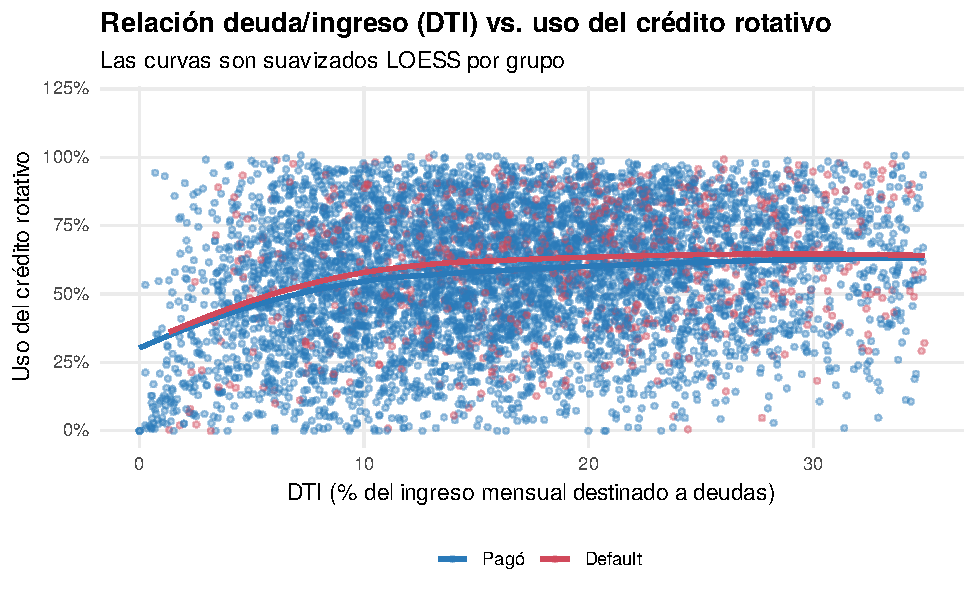
\includegraphics[width=0.49\textwidth]{eda_scatter_dti_revol.pdf}
  \caption{Diagramas de dispersión de una muestra de 6.000 préstamos de
  entrenamiento. Izquierda: tasa de interés vs. ingreso anual. Derecha: DTI vs.
  uso del crédito rotativo, con suavizado LOESS por grupo.}
  \label{fig:scatter-eda}
\end{figure}

El propósito del préstamo también importa (Figura~\ref{fig:proposito}): los
préstamos para pequeñas empresas son los más riesgosos (22\% de default), y los
destinados a autos, compras grandes o pagar tarjetas de crédito, los menos
riesgosos (10\%--11\%).

\begin{figure}[htbp]
  \centering
  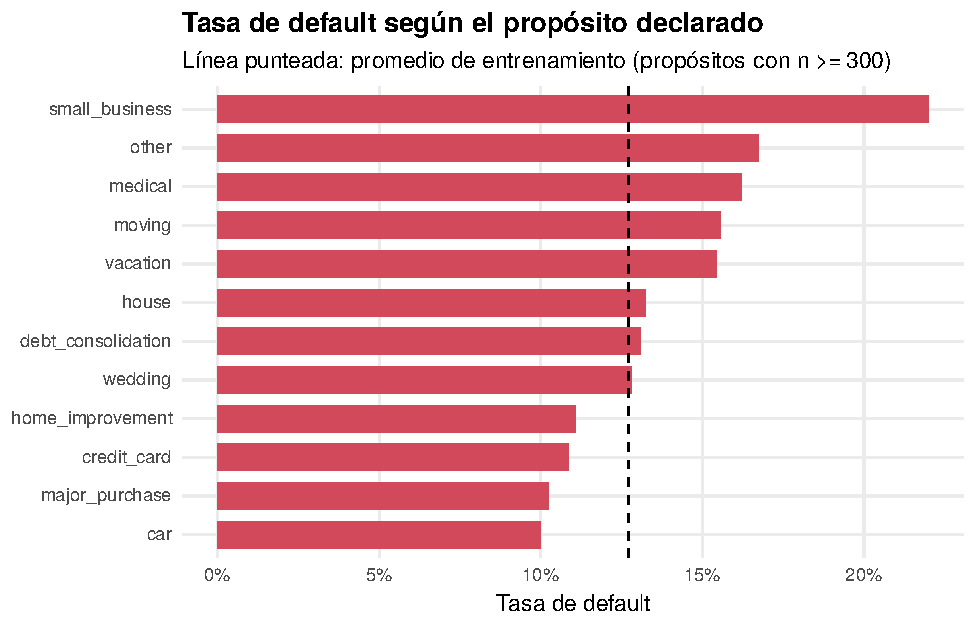
\includegraphics[width=0.8\textwidth]{eda_default_proposito.pdf}
  \caption{Tasa de default según el propósito declarado (entrenamiento).}
  \label{fig:proposito}
\end{figure}

La Figura~\ref{fig:faltantes} cuantifica los datos faltantes, que motivan las dos
estrategias de imputación, y la Figura~\ref{fig:correlacion} muestra
correlaciones casi perfectas, como monto y cuota ($r=\corrCuotaMonto$), que
justifican el filtro de correlación.

\begin{figure}[htbp]
  \centering
  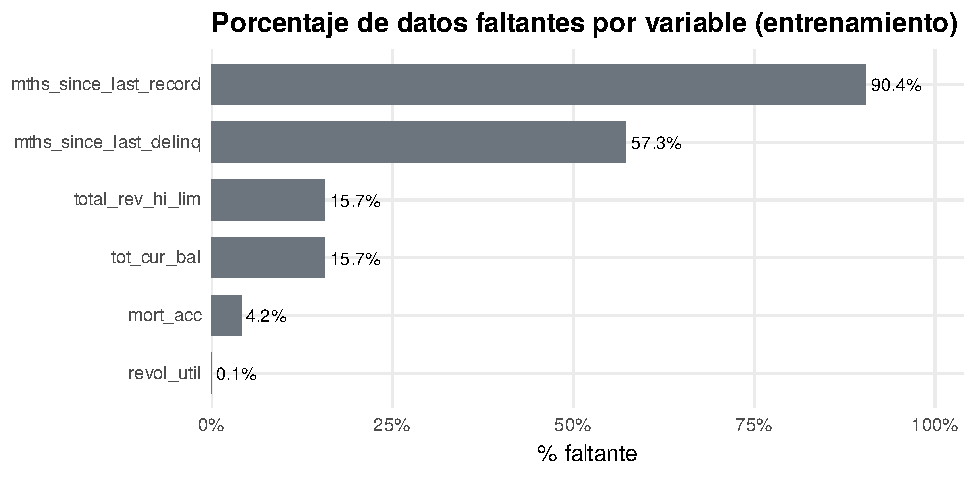
\includegraphics[width=0.8\textwidth]{eda_faltantes.pdf}
  \caption{Porcentaje de datos faltantes por variable (entrenamiento).}
  \label{fig:faltantes}
\end{figure}

\begin{figure}[htbp]
  \centering
  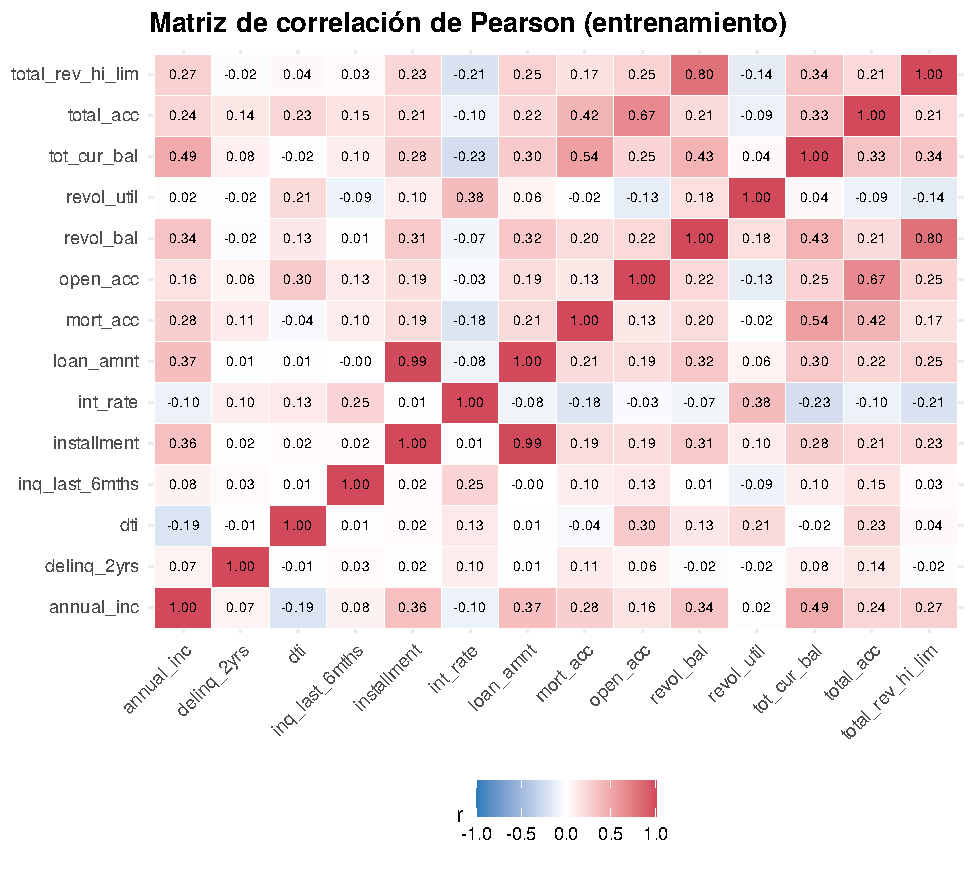
\includegraphics[width=0.72\textwidth]{eda_correlacion.pdf}
  \caption{Matriz de correlación de Pearson entre variables numéricas.}
  \label{fig:correlacion}
\end{figure}

\FloatBarrier
\subsection{Selección de características}

De \nCandidatas{} características candidatas, \nDescIV{} se descartaron por
IV $< 0{,}02$ y \nDescCor{} por correlación (Figura~\ref{fig:iv} y
Tabla~\ref{tab:iv}). Se destacan tres resultados:
\begin{itemize}
  \item El sub-grado (IV $=\ivSubgrado$) y la tasa de interés (IV $=\ivTasa$) son
        las variables más predictivas, pero tienen $|r|=0{,}99$ entre sí, porque
        LendingClub fija la tasa según el sub-grado. Se conservó el sub-grado.
  \item Dos variables \textbf{creadas por ingeniería de características},
        \texttt{dti\_con\_prestamo} y \texttt{cuota\_ingreso}, quedaron cuarta
        y quinta en IV y \emph{reemplazaron} a las originales (\texttt{dti} y
        \texttt{prestamo\_ingreso}) en el filtro de correlación.
  \item Variables que intuitivamente parecerían importantes, como los atrasos de
        los últimos dos años o los registros públicos negativos, tienen IV casi
        nulo. LendingClub ya filtra a los solicitantes con mal historial, así
        que entre los aprobados esas variables casi no varían.
\end{itemize}
Quedaron \nFinales{} variables (incluidos 4 indicadores de faltante), que generan
\nColumnasX{} columnas en la matriz de diseño. El LASSO llevó a cero
\lassoCeros{} de esos \lassoTotal{} coeficientes: las variables de saldos y uso
del crédito (saldo total, límite rotativo, uso del rotativo e hipotecas), cuya
información ya está contenida en el ingreso y el endeudamiento; la mayoría de las
categorías de propósito y vivienda (sólo sobrevivieron \emph{pequeña empresa},
\emph{tarjeta de crédito} y \emph{alquila}, medidas respecto de las categorías
de referencia \emph{auto} e \emph{hipoteca}), y dos indicadores de faltante.

\begin{figure}[htbp]
  \centering
  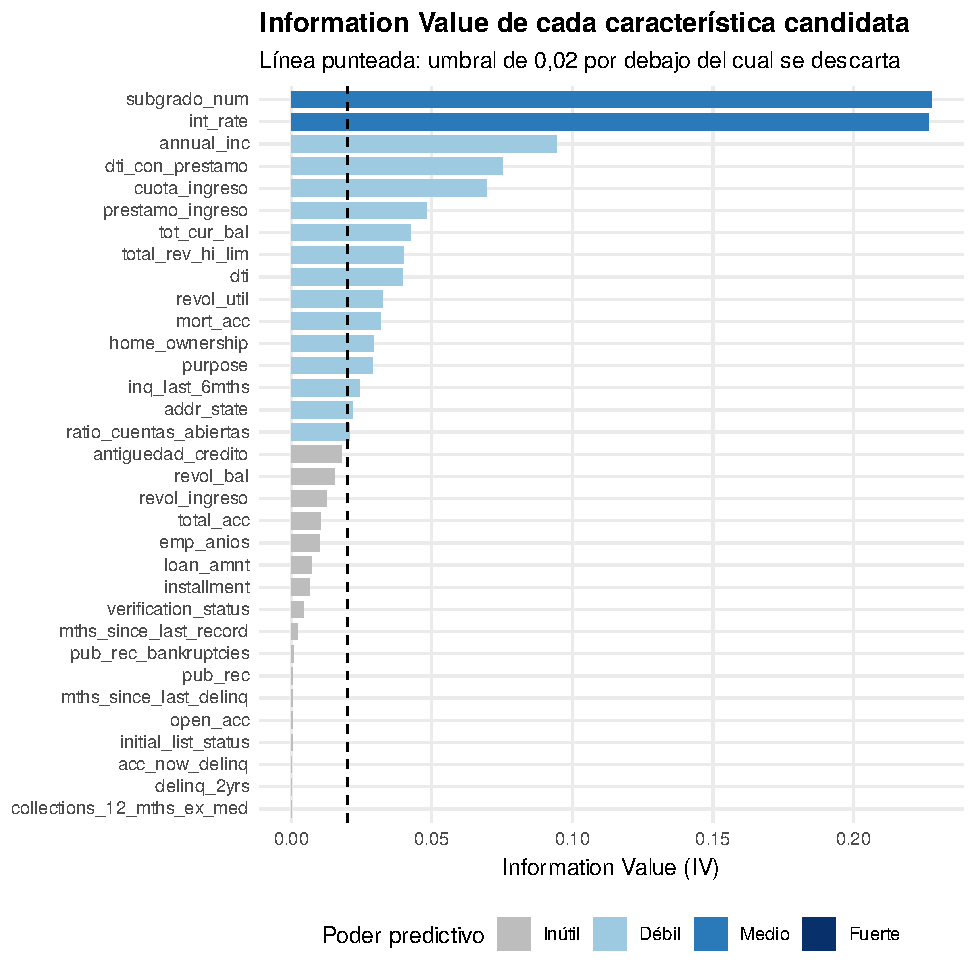
\includegraphics[width=0.78\textwidth]{features_information_value.pdf}
  \caption{Information Value de las \nCandidatas{} características candidatas.
  La línea punteada marca el umbral de descarte.}
  \label{fig:iv}
\end{figure}

\begin{table}[htbp]
\caption{Information Value por característica (calculado en el conjunto de ajuste).}
\label{tab:iv}
\centering
\small
\begin{tabular}{lrl}
\toprule
Variable & IV & Poder predictivo \\
\midrule
\tablainput{../results/tabla_iv.tex}
\bottomrule
\end{tabular}
\end{table}

\FloatBarrier
\subsection{Desempeño de los modelos}

La Figura~\ref{fig:tuning} muestra la búsqueda de hiperparámetros de Gradient
Boosting en validación. El AUC alcanza su máximo con pocos árboles y luego baja
levemente: más árboles sobreajustan patrones del período de entrenamiento que no
se repiten en el siguiente.

\begin{figure}[htbp]
  \centering
  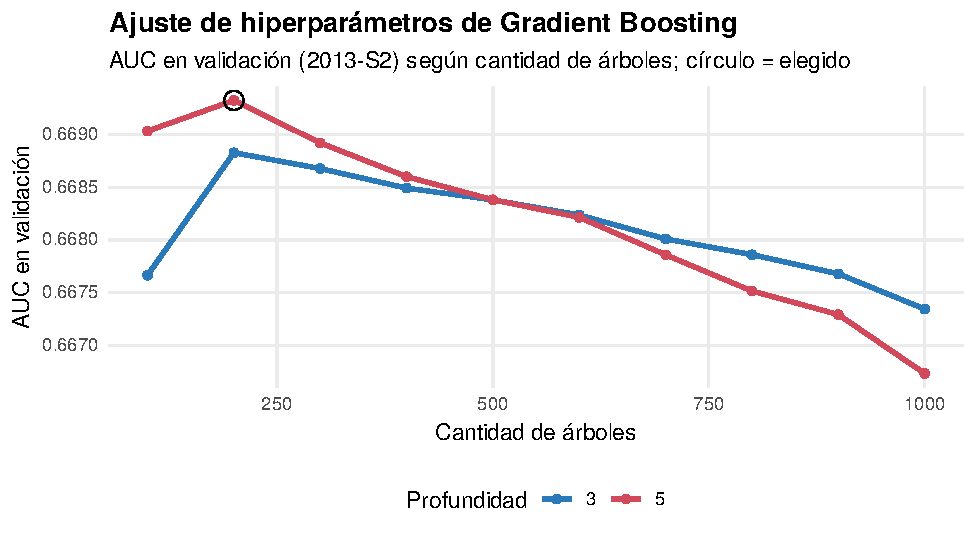
\includegraphics[width=0.75\textwidth]{modelo_tuning_gbm.pdf}
  \caption{AUC en validación de Gradient Boosting según profundidad y cantidad de
  árboles.}
  \label{fig:tuning}
\end{figure}

La Tabla~\ref{tab:metricas} resume el desempeño en el conjunto de prueba
(2014-S1), que no se usó para ninguna decisión. El modelo principal
(\mejorModelo) se eligió por su AUC en \emph{validación}, no en prueba.

\begin{table}[htbp]
\caption{Desempeño en prueba (\nTest{} préstamos de 2014-S1). AUC con intervalo de
confianza de 95\% (DeLong). Las métricas de la derecha usan el umbral elegido en
validación (Youden). Sombreado: modelo principal.}
\label{tab:metricas}
\centering
\resizebox{\textwidth}{!}{%
\begin{tabular}{lccccccccc}
\toprule
Modelo & AUC valid. & AUC prueba [IC 95\%] & Gini & KS & Brier & Accuracy & Sensib. & Especif. & F1 \\
\midrule
\tablainput{../results/tabla_metricas.tex}
\bottomrule
\end{tabular}}
\end{table}

\begin{figure}[htbp]
  \centering
  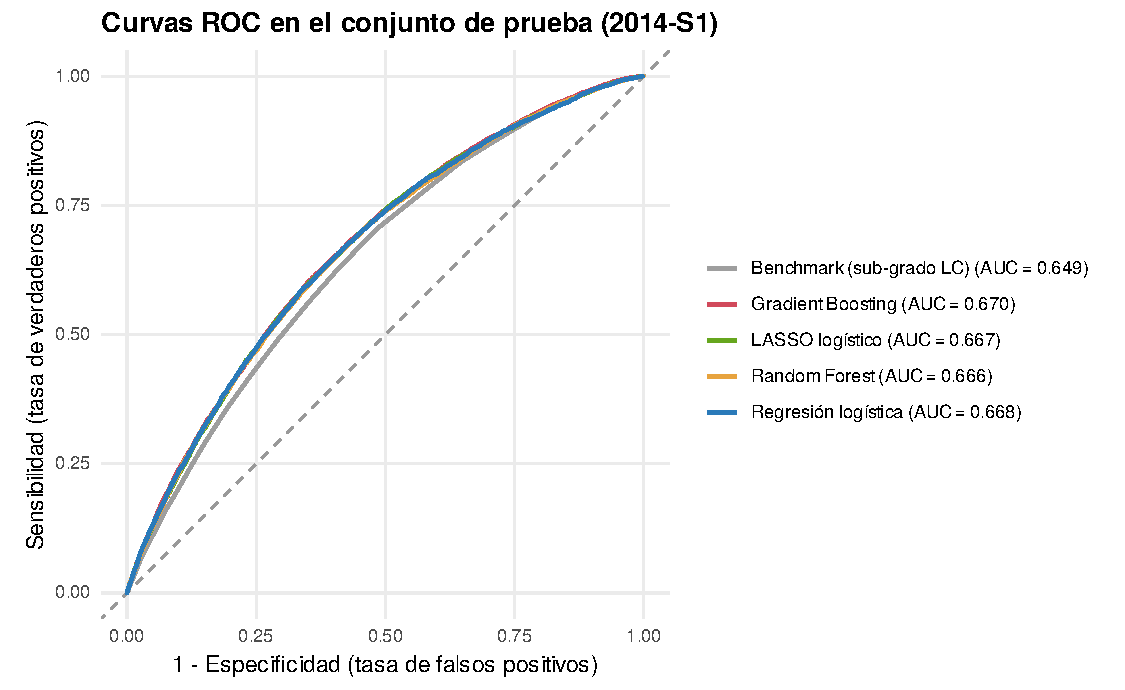
\includegraphics[width=0.9\textwidth]{resultado_roc.pdf}
  \caption{Curvas ROC de los cinco modelos en el conjunto de prueba.}
  \label{fig:roc}
\end{figure}

Los resultados principales son:
\begin{enumerate}
  \item \textbf{Todos los modelos superan a la calificación de LendingClub.}
        \mejorModelo{} obtiene un AUC de \aucMejor{} (Gini \giniMejor) frente a
        \aucBench{} (Gini \giniBench) del benchmark. La diferencia es
        estadísticamente significativa (DeLong, $p=$ \pDelongBench). En la
        Figura~\ref{fig:roc} la curva del benchmark queda por debajo de las demás
        en prácticamente todo el rango.
  \item \textbf{La complejidad aporta poco.} La regresión logística
        (AUC \aucLogit) queda a milésimas de Gradient Boosting. La diferencia es
        significativa ($p=\pDelongLogit$) por el gran tamaño de muestra, pero es
        prácticamente irrelevante. Esto coincide con \citet{namvar2018},
        \citet{turiel2020} y con la comparación general de \citet{lessmann2015}:
        en datos tabulares de crédito, la mayor parte de la ganancia viene de las
        variables, no del algoritmo.
  \item \textbf{Estabilidad temporal.} El AUC de validación (2013-S2) y el de
        prueba (2014-S1) son casi idénticos en todos los modelos. Los modelos
        generalizan a un período nuevo sin degradarse.
  \item \textbf{El \emph{accuracy} engaña.} Un clasificador trivial que dice
        ``todos pagan'' tendría un \emph{accuracy} cercano a 86,8\% (1 menos la
        tasa de default de prueba) y no detectaría ni un solo default. Con el
        umbral de Youden, \mejorModelo{} tiene un \emph{accuracy} de \accMejor,
        pero detecta el \sensMejor{} de los defaults (sensibilidad) y conserva el
        \especMejor{} de los buenos pagadores (especificidad).
\end{enumerate}

\paragraph{Matriz de confusión.} La Figura~\ref{fig:confusion} compara el
benchmark con el modelo principal. Con un umbral de \umbralMejor{}, \mejorModelo{}
detecta más defaults \emph{y} rechaza menos buenos pagadores que el benchmark:
mejora ambos tipos de error a la vez. La precisión es baja (\precMejor), es decir,
de cada 100 préstamos señalados como riesgosos, unos 19 terminan en default. Es
inevitable cuando la clase positiva es minoritaria y las clases se superponen
tanto (Figura~\ref{fig:scatter-eda}). La Tabla~\ref{tab:umbral} muestra el umbral
y las métricas complementarias de cada modelo.

\begin{figure}[htbp]
  \centering
  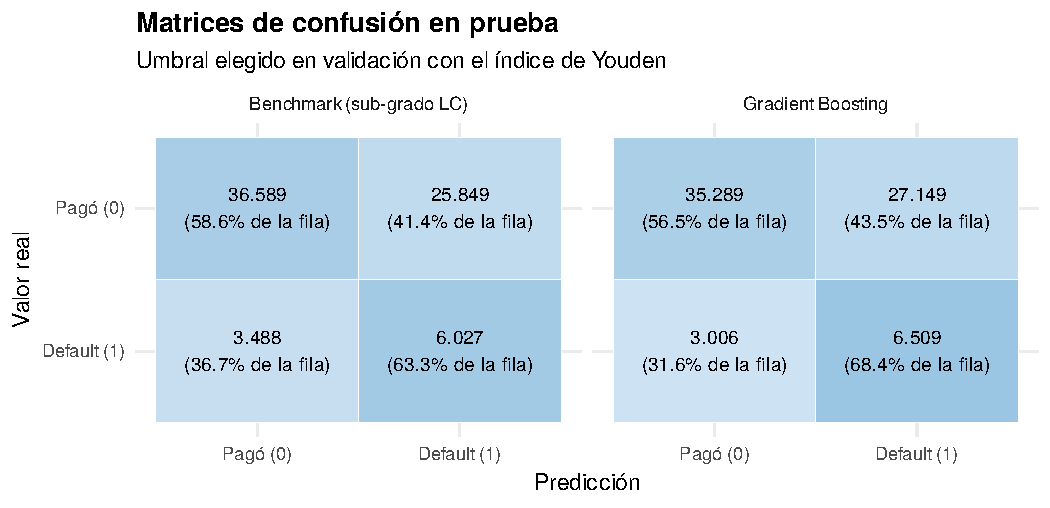
\includegraphics[width=0.92\textwidth]{resultado_matriz_confusion.pdf}
  \caption{Matrices de confusión en prueba con el umbral elegido en validación.}
  \label{fig:confusion}
\end{figure}

\begin{table}[htbp]
\caption{Umbral de decisión (elegido en validación) y métricas complementarias en
prueba.}
\label{tab:umbral}
\centering
\begin{tabular}{lcccc}
\toprule
Modelo & Umbral & Precisión & Accuracy balanceada & F1 \\
\midrule
\tablainput{../results/tabla_metricas_umbral.tex}
\bottomrule
\end{tabular}
\end{table}

\FloatBarrier
\subsection{Calibración y separación de clases}

Para fijar precios o provisiones, no alcanza con ordenar bien a los clientes:
la probabilidad estimada tiene que coincidir con la frecuencia real. La
Figura~\ref{fig:calibracion} muestra que todos los modelos están bien calibrados
(los puntos siguen la diagonal), con una leve subestimación en los deciles de
mayor riesgo. El benchmark es el que peor separa los extremos: su decil más
riesgoso tiene menos defaults que el de los demás modelos. La
Figura~\ref{fig:densidad} muestra la superposición de las distribuciones de score
(KS $=\ksMejor$).

\begin{figure}[htbp]
  \centering
  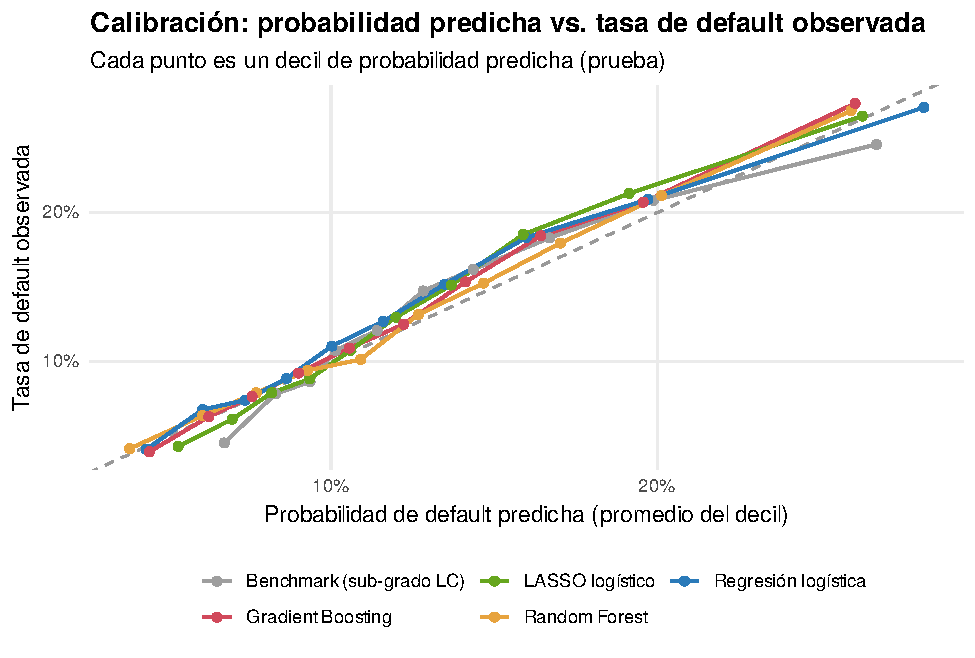
\includegraphics[width=0.8\textwidth]{resultado_calibracion.pdf}
  \caption{Curvas de calibración por deciles de probabilidad predicha (prueba).}
  \label{fig:calibracion}
\end{figure}

\begin{figure}[htbp]
  \centering
  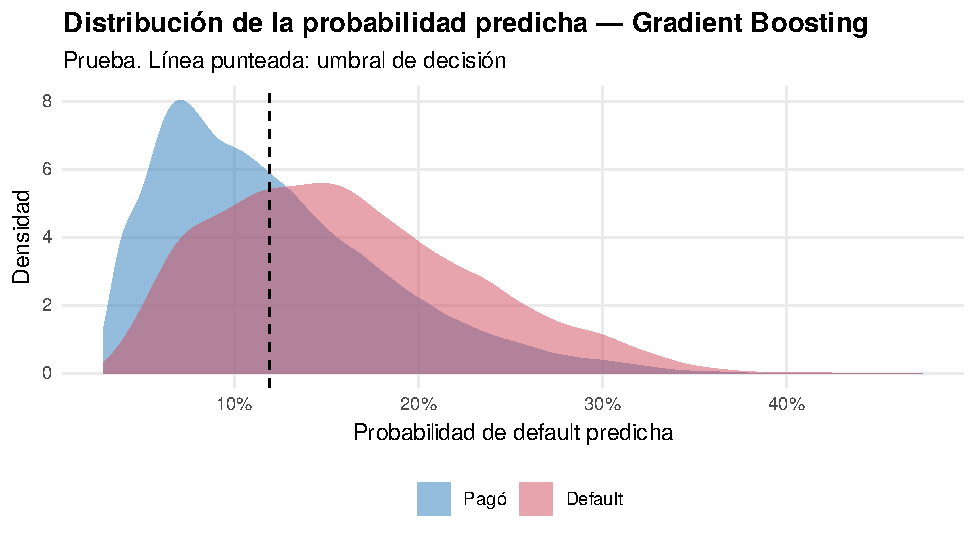
\includegraphics[width=0.8\textwidth]{resultado_densidad_scores.pdf}
  \caption{Distribución de la probabilidad predicha por \mejorModelo{} según el
  resultado real.}
  \label{fig:densidad}
\end{figure}

\FloatBarrier
\subsection{Interpretación: ¿qué explica el default?}

La Figura~\ref{fig:or} y la Tabla~\ref{tab:coef} muestran los coeficientes de la
regresión logística. Como las variables están estandarizadas, sus efectos se
pueden comparar entre sí. Un desvío estándar más de sub-grado multiplica las
chances de default por 1,41. Un desvío más de ingreso las reduce un 15\%. Más
endeudamiento (incluido el préstamo nuevo), más consultas de crédito recientes
y destinar el préstamo a una pequeña empresa aumentan el riesgo. Todos los signos
tienen sentido económico.

\begin{figure}[htbp]
  \centering
  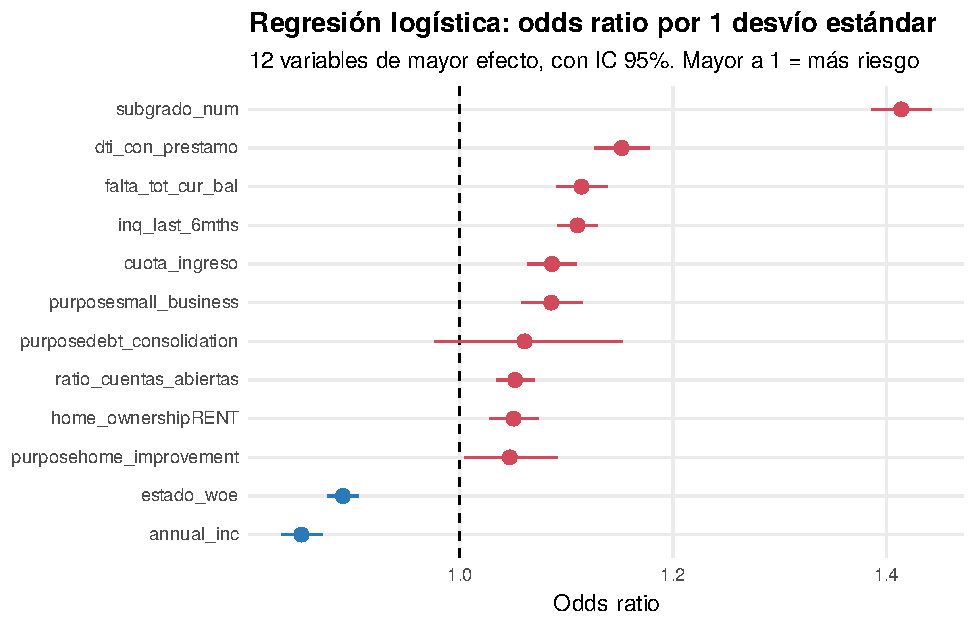
\includegraphics[width=0.8\textwidth]{resultado_odds_ratios.pdf}
  \caption{Odds ratios de la regresión logística (por un desvío estándar) con
  intervalos de confianza de 95\%.}
  \label{fig:or}
\end{figure}

\begin{table}[htbp]
\caption{Las 10 variables de mayor efecto en la regresión logística (variables
estandarizadas).}
\label{tab:coef}
\centering
\begin{tabular}{lrrr}
\toprule
Variable & $\hat\beta$ & Odds ratio & $p$-valor \\
\midrule
\tablainput{../results/tabla_coeficientes.tex}
\bottomrule
\end{tabular}
\end{table}

Los modelos de árboles coinciden en las variables principales
(Figura~\ref{fig:importancia}): sub-grado, ingreso, DTI con préstamo y cuota sobre
ingreso. Dos de esas cuatro variables fueron creadas en este trabajo.

\begin{figure}[htbp]
  \centering
  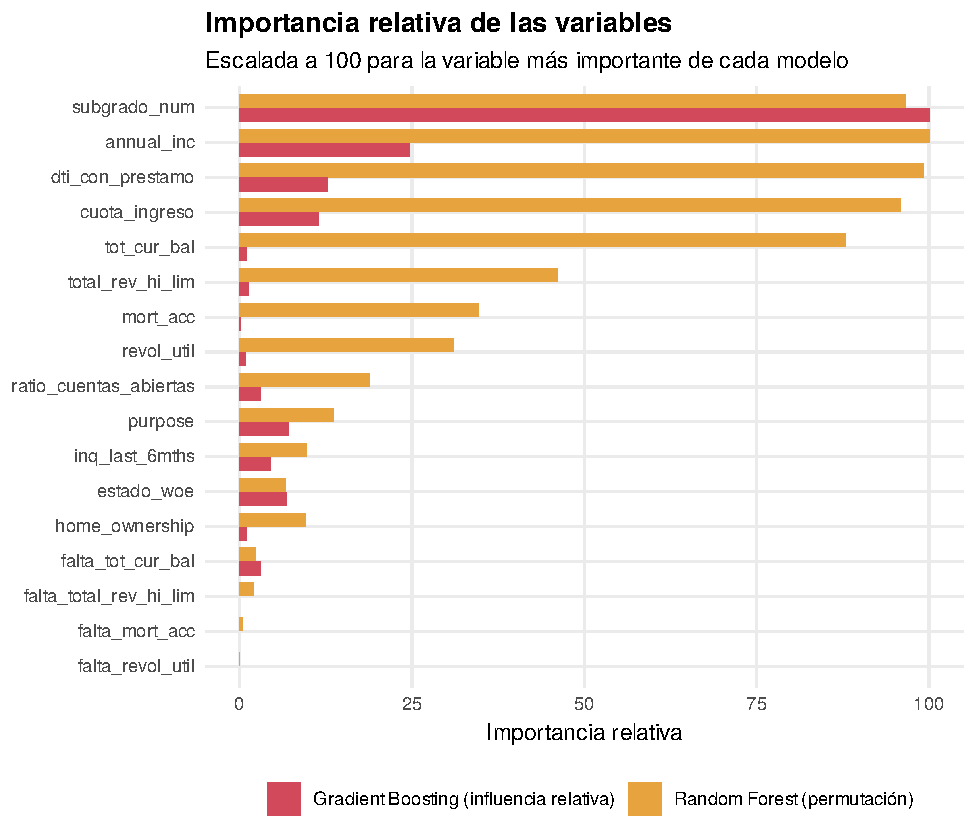
\includegraphics[width=0.8\textwidth]{resultado_importancia.pdf}
  \caption{Importancia relativa de las variables en Random Forest (permutación) y
  Gradient Boosting (influencia relativa).}
  \label{fig:importancia}
\end{figure}

La Figura~\ref{fig:scatter-pd} compara el riesgo estimado por el modelo con la
tasa que cobró LendingClub. La correlación de Spearman es alta (\corrTasaPD),
porque el sub-grado es la variable principal del modelo. La dispersión vertical
dentro de cada nivel de tasa es justamente el valor agregado del modelo: entre
dos clientes a los que LendingClub cobró la misma tasa, el modelo distingue cuál
es más riesgoso.

\begin{figure}[htbp]
  \centering
  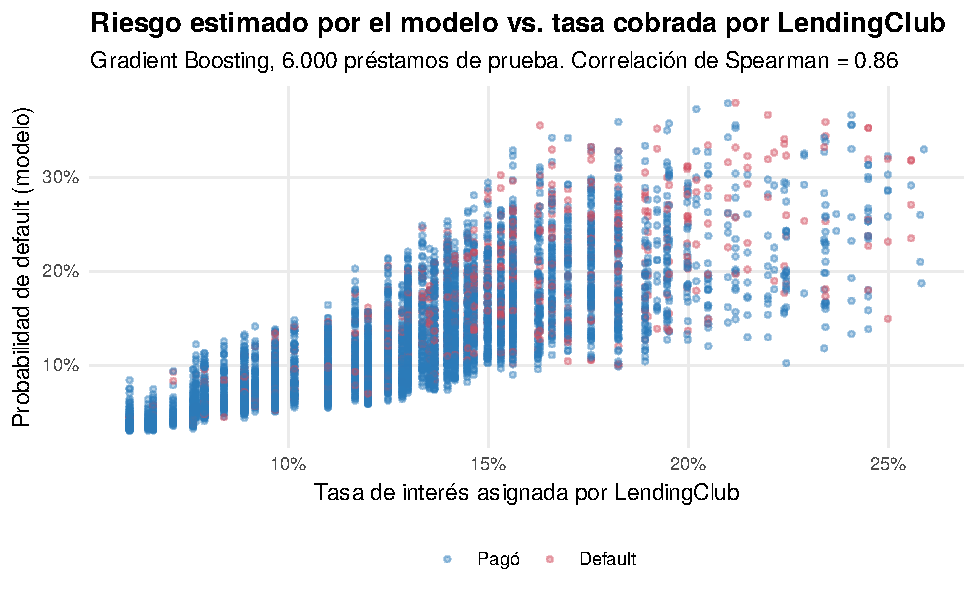
\includegraphics[width=0.85\textwidth]{resultado_scatter_pd_tasa.pdf}
  \caption{Probabilidad de default estimada vs. tasa de interés asignada por
  LendingClub (6.000 préstamos de prueba).}
  \label{fig:scatter-pd}
\end{figure}

\FloatBarrier
\subsection{Impacto económico}
\label{sec:res-eco}

La Figura~\ref{fig:economico} y la Tabla~\ref{tab:economica} traducen los
resultados a dinero, con lo que realmente se cobró de cada préstamo de prueba.

\begin{figure}[htbp]
  \centering
  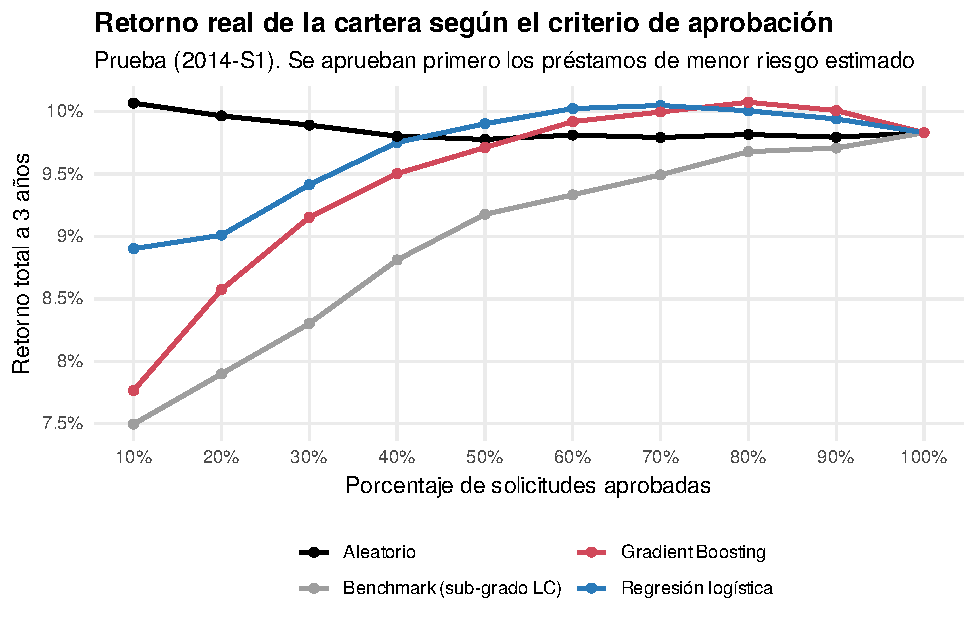
\includegraphics[width=0.85\textwidth]{resultado_economico.pdf}
  \caption{Retorno real a 3 años de la cartera aprobada según el criterio y la tasa
  de aprobación (prueba).}
  \label{fig:economico}
\end{figure}

\begin{table}[htbp]
\caption{Tasa de default y retorno real a 3 años de la cartera aprobada (prueba).}
\label{tab:economica}
\centering
\begin{tabular}{cccccc}
\toprule
& \multicolumn{3}{c}{Tasa de default de la cartera} & \multicolumn{2}{c}{Retorno a 3 años} \\
\cmidrule(lr){2-4}\cmidrule(lr){5-6}
Aprobación & Aleatorio & Sub-grado LC & \mejorModelo & Sub-grado LC & \mejorModelo \\
\midrule
\tablainput{../results/tabla_economica.tex}
\bottomrule
\end{tabular}
\end{table}

\begin{itemize}
  \item \textbf{Con el mismo volumen, mejor cartera.} Aprobando el 70\% de las
        solicitudes, el modelo arma una cartera con \defMejorSetenta{} de default
        (contra \defBenchSetenta{} ordenando por sub-grado) y retorno de
        \retMejorSetenta{} (contra \retBenchSetenta). Sobre la cartera de prueba,
        eso equivale a US\$\difGanSetenta{} más de ganancia (US\$\ganMejorSetenta{}
        contra US\$\ganBenchSetenta) prestando la misma cantidad de préstamos.
  \item \textbf{Minimizar defaults no es lo mismo que maximizar ganancia.} Es el
        hallazgo más contraintuitivo. Aprobar sólo el 10\% más seguro según el
        sub-grado rinde 7,5\%, \emph{menos} que aprobar al azar (10,1\%), porque
        los clientes más seguros pagan tasas muy bajas. Los modelos predictivos
        evitan parte de esta trampa porque ordenan por riesgo \emph{dentro} de
        cada nivel de tasa, pero tampoco maximizan la ganancia. Esto confirma la
        advertencia de \citet{xia2017}: un modelo de \emph{default} no es un
        modelo de \emph{rentabilidad}.
  \item \textbf{Prestar a todos fue rentable en este período.} Aprobando el 100\%,
        el retorno fue de \retTodos{} (US\$\ganTodos{} sobre la cartera de prueba).
        En términos absolutos, rechazar préstamos reduce la ganancia total
        aunque mejore el retorno porcentual. El valor del modelo depende del
        objetivo del inversor (rendimiento por dólar invertido o volumen) y del
        costo de oportunidad del capital.
\end{itemize}

\subsection{Experimento: el espejismo de la fuga de información}
\label{sec:res-fuga}

Para mostrar por qué la prevención de fuga es la decisión metodológica más
importante del trabajo, se re-entrenó la regresión logística agregando tres
variables que \emph{sólo existen después de otorgar el préstamo}: la proporción
de capital devuelto, si hubo recuperos y el monto del último pago. El AUC en
prueba saltó a \aucFuga{} (Figura~\ref{fig:fuga}): el modelo es ``casi perfecto''
pero completamente inútil, porque el día de la solicitud esas variables no
existen. Este experimento brinda una explicación plausible para los resultados
de AUC superiores a 0,90 que aparecen en parte de la literatura
\cite{gupta2022}, y muestra que con datos de LendingClub un AUC cercano a 0,70 no
es un mal resultado sino el techo realista con información de originación.

\begin{figure}[htbp]
  \centering
  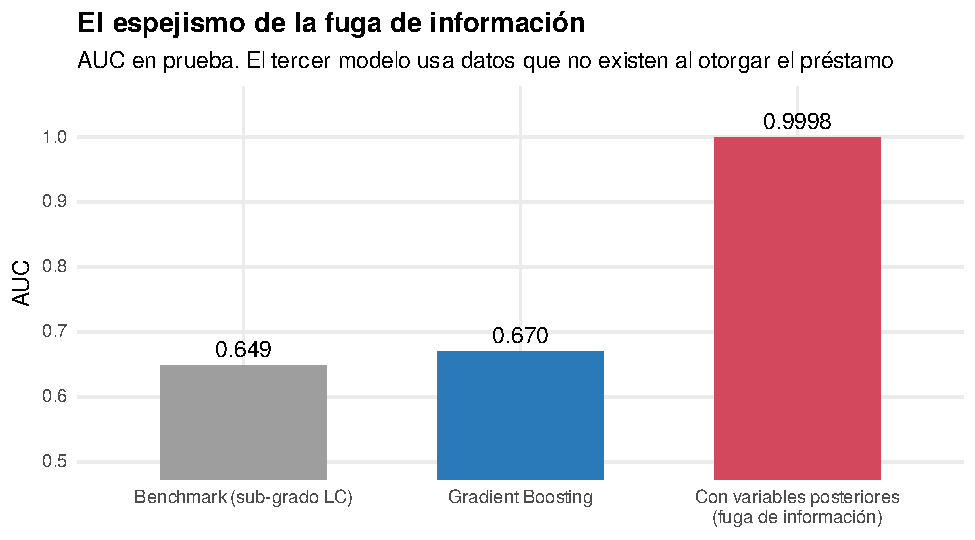
\includegraphics[width=0.78\textwidth]{resultado_fuga_informacion.pdf}
  \caption{AUC en prueba del benchmark, del modelo principal y de un modelo con
  variables posteriores al otorgamiento (fuga de información).}
  \label{fig:fuga}
\end{figure}

\FloatBarrier
\subsection{Comparación con el estado del arte}

El AUC obtenido (\aucMejor) es algo menor que el de \citet{namvar2018} (0,69--0,71)
y \citet{turiel2020} (0,69). Las diferencias tienen explicación:
(i) la evaluación es estrictamente fuera de tiempo y con todas las decisiones
tomadas antes de ver la prueba, mientras que \citet{namvar2018} usan una
partición aleatoria; (ii) se restringió a préstamos a 36 meses, una población más
homogénea y de menor riesgo, en la que discriminar es más difícil; y (iii) la
versión de los datos utilizada no incluye el puntaje FICO, que
\citet{emekter2015} y \citet{malekipirbazari2015} identifican como uno de los
predictores principales. Por otro lado, el resultado coincide con la literatura
en que el grado de LendingClub es la variable más informativa
\cite{serrano2015,emekter2015}, en que los modelos de aprendizaje automático lo
superan \cite{malekipirbazari2015}, y en que la regresión logística compite de
igual a igual con métodos más complejos \cite{namvar2018,turiel2020}.

% =====================================================================
\section{Conclusiones}
\label{sec:conclusiones}

Se construyó un modelo de riesgo de crédito sobre \nTotal{} préstamos reales de
LendingClub con un protocolo libre de fuga de información y validación fuera de
tiempo. El mejor modelo (\mejorModelo, AUC \aucMejor) supera de manera
estadísticamente significativa a la calificación de la propia plataforma
(AUC \aucBench). Con el mismo volumen de aprobación, arma una cartera con menos
defaults y más retorno. La ingeniería de características aportó dos de las cuatro
variables más importantes, y el experimento de fuga mostró que métricas casi
perfectas en este problema son una señal de alarma y no de éxito.

\paragraph{Pros.}
\begin{itemize}
  \item Datos reales, abundantes y con resultado definitivo, sin sesgo de
        préstamos todavía vigentes.
  \item Validación honesta: partición temporal, hiperparámetros y umbral elegidos
        fuera de tiempo y prueba usada una sola vez.
  \item Resultados estables entre validación y prueba, modelos bien calibrados e
        interpretables (signos con sentido económico).
  \item Evaluación económica con dinero efectivamente cobrado, no sólo métricas
        estadísticas.
  \item Código completamente reproducible: cada número del informe sale del
        código.
\end{itemize}

\paragraph{Contras y limitaciones.}
\begin{itemize}
  \item La mejora sobre la calificación de LendingClub es real pero moderada
        (+0,02 de AUC). Los modelos complejos casi no superan a la regresión
        logística.
  \item \textbf{Sesgo de selección (\emph{reject inference}).} Sólo se observan
        préstamos \emph{aprobados}. No se sabe cómo se habrían comportado los
        rechazados, así que el modelo no puede usarse tal cual para decidir sobre
        toda la población de solicitantes.
  \item La versión de los datos no incluye el puntaje FICO, ni texto, ni
        variables macroeconómicas.
  \item El análisis económico es bruto: no descuenta comisiones, costo de fondeo
        ni el valor tiempo del dinero, y supone que el inversor puede elegir
        qué préstamos financiar.
  \item El período de prueba (2014) fue de expansión económica. El desempeño en
        una recesión podría ser distinto.
\end{itemize}

\paragraph{Trabajos futuros.}
\begin{itemize}
  \item \textbf{Modelar la rentabilidad, no sólo el default}: estimar la ganancia
        esperada $E[\text{ganancia}] = (1-\hat p)\cdot\text{interés} -
        \hat p \cdot \text{pérdida}$, o entrenar directamente modelos sensibles
        al costo \cite{xia2017}.
  \item Incorporar el puntaje FICO y probar XGBoost/LightGBM \cite{ma2018}.
  \item Modelos de supervivencia, que predicen \emph{cuándo} ocurre el default y
        aprovechan los préstamos todavía vigentes \cite{emekter2015}.
  \item Técnicas de \emph{reject inference} para corregir el sesgo de selección.
  \item Explicabilidad local (por ejemplo, valores SHAP) para justificar cada
        decisión individual ante el solicitante y el regulador.
  \item Evaluar la equidad del modelo entre grupos (por ejemplo, por estado de
        residencia) y su estabilidad en períodos de crisis.
\end{itemize}

% =====================================================================
\section*{Reproducibilidad}
El proyecto completo (datos, código R comentado con pre/postcondiciones e
invariantes, figuras y este informe) se ejecuta abriendo
\texttt{LendingClub\_RiesgoCredito.Rproj} en RStudio y corriendo
\texttt{main.R}. Las librerías utilizadas son \texttt{ggplot2}, \texttt{pROC}
\cite{robin2011}, \texttt{glmnet} \cite{friedman2010}, \texttt{ranger}
\cite{wright2017} y \texttt{gbm}. La semilla aleatoria está fija, de modo que
los resultados son idénticos en cualquier PC.

\bibliographystyle{unsrtnat}
\bibliography{references}

\end{document}
